\documentclass{zc-ust-hw}

\usepackage{lipsum}

\name{SalahDin Ahmed Salh Rezk}
\id{202201079}
\course{Digital Design and Computer Architecture (CIE 239)}
\assignment{Assignment 3}

\begin{document}

\maketitle

\begin{enumerate}

  \item If all the inputs $P$, $Q$, $R$, $S$ and $T$ are applied simultaneously and held
    constant. Determine the propagation delay and contamination delay of the
    following circuit. Use the gate delays given. the XOR gate, AND gate and
    multiplexer (MUX) are 4 ns, 2 ns and 1 ns, respectively. 

    \begin{sol}
      \begin{align}
        Pd &= Pd_{\text{XOR}} + Pd_{\text{MUX}} + Pd_{\text{AND}} + Pd_{\text{MUX}} = 4 + 1 + 2 + 1 = 8 \text{ ns} \\
        Cd &= Cd_{\text{AND}} + Cd_{\text{MUX}} = 2 + 1 = 3 \text{ ns}
      .\end{align}
    \end{sol}

  \item Write a minimized Boolean equation for the function performed by the
    circuit and Implement the function using a 2:1 multiplexer and other logic
    gates. 

    \begin{sol} \,
    \begin{table}[H]
      \begin{center}
        \begin{tabular}{c|c|c}
          \( s_{1} \) & \( s_{0} \) & out \\ 
          \hline
          0 & 0 & \( i_{0} \) \\
          0 & 1 & \( i_{1} \) \\
          1 & 0 & \( i_{2} \) \\
          1 & 1 & \( i_{3} \) \\
        \end{tabular}
      \end{center}
      \caption{}
    \end{table}
    \begin{align}
    \text{out} = \overline{s_{1}} \overline{s_{0}} i_{0} + \overline{s_{1}} s_{0} i_{1} + s_{1} \overline{s_{0}} i_{2} + s_{1} s_{0} i_{3}
    .\end{align}
    \( \implies \) when \( s_{1}=0 \), the output of \( m_{1} \) is selected. When \( s_{1}=1 \), the output of \( m_{2} \) is selected.
    \begin{figure}[H]
      \begin{center}
        \begin{circuitikz}[american]
          % Nodes
          \node (s0) at (0, 0) {\( s_{0} \)};
          % MUX
          \draw (s0) ++(3, -1) node[muxdemux, muxdemux def={Lh=2, NL=2, Rh=1,NB=1, w=1, square pins=1}] (mux1) {};
          % Not
          \draw (mux1.lpin 2) ++(-1, 0) node[not port, scale=0.5] (not1) {};
          % Connections
          \draw (mux1.lpin 1)  to[short, -*] (0, |- mux1.lpin 1);
          \draw (mux1.lpin 2)  to[short] (not1.out);
          \draw (not1.in)      to[short, -*] (0, |- mux1.lpin 2);
          % Lines
          \draw (s0) -- ++(0, |-mux1.lpin 2) {};
          % Labels
          \node at (mux1.bpin 1) [below] {\( s_{1} \)};
        \end{circuitikz}
      \end{center}
      \caption{}
    \end{figure}
    \end{sol}

    \newpage
    
  \item Given the input waveforms shown in figure below, sketch the output $Q$
    of an SR latch. 

    \begin{sol} \,
      \begin{figure}[H]
        \begin{center}
          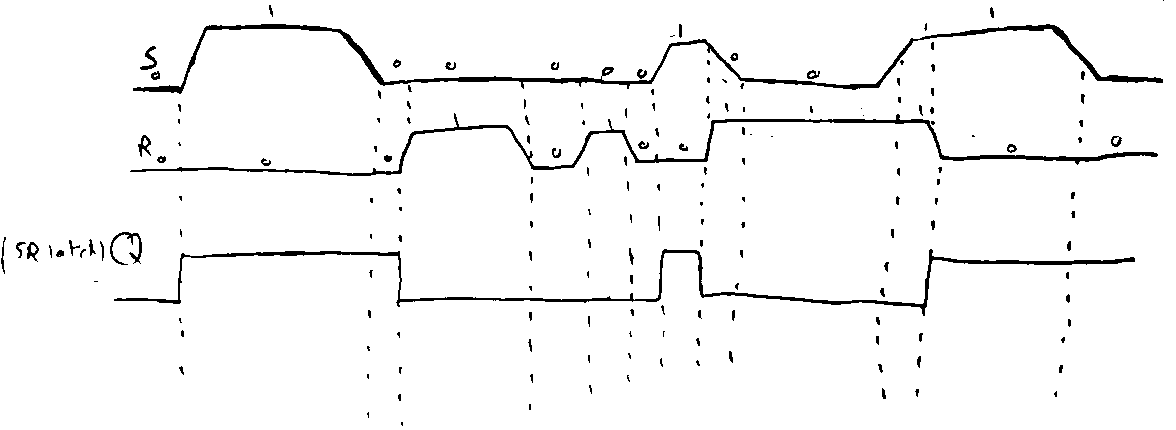
\includegraphics[width=0.95\textwidth]{figures/1702587458.png}
        \end{center}
        \caption{}
      \end{figure}
    \end{sol}

    \item Given the input waveforms shown in figure below, sketch the output,
      Q, of D latch and D flip-flop.

      \begin{sol} \,
        \begin{figure}[H]
          \begin{center}
            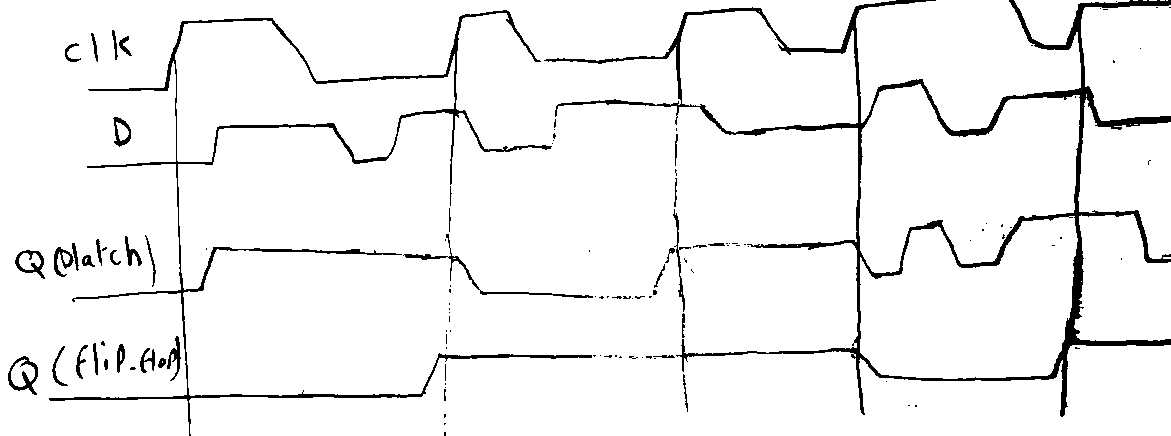
\includegraphics[width=0.95\textwidth]{figures/1702587611.png}
          \end{center}
          \caption{}
        \end{figure}
      \end{sol}

      \newpage
       
    \item The following characteristic table describes a storage element A--B

      \begin{enumerate}
        \item Write the characteristic equation for the storage element A--B.
          \begin{sol}
            \begin{align}
              Q_{n+1} &= aL \overline{Q}_n + \overline{L} Q_n \\
              S &= aL \overline{Q}\\
              R &= L Q
            .\end{align}
          \end{sol}

        \item Implement the A--B storage element using additional gates and an
          S--R Latch. Show your schematic diagram and derivation process. 

          \begin{sol} \,
            \begin{table}[H]
              \begin{center}
                \begin{tabular}{c|c|c||c|c|c}
                  \( a \) & \( L \) & \( Q_{n} \) & \( Q_{n+1} \) & \( S \) & \( R \) \\
                  \hline
                  0 & 0 & 0 & 0 & 0 & X \\
                  0 & 0 & 1 & 1 & X & 0 \\
                  0 & 1 & 0 & 0 & 0 & X \\
                  0 & 1 & 1 & 0 & 0 & 1 \\
                  1 & 0 & 0 & 0 & 0 & X \\
                  1 & 0 & 1 & 1 & X & 0 \\
                  1 & 1 & 0 & 1 & 1 & 0 \\
                  1 & 1 & 1 & 0 & 0 & 1 \\
                \end{tabular}
              \end{center}
              \caption{}
            \end{table}

            \begin{figure}[H]
              \begin{center}
                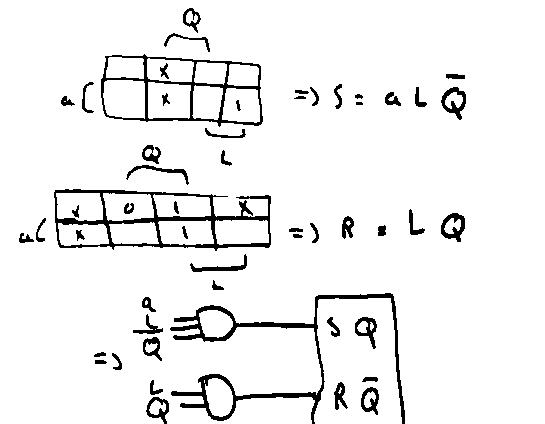
\includegraphics[width=0.70\textwidth]{figures/1702588363.png}
              \end{center}
              \caption{}
            \end{figure}
          \end{sol}
      \end{enumerate}

      \newpage

    \item Construct a JK flip-flop using a D flip-flop, a two-to-one-line
      multiplexer, and an inverter.

      \begin{sol} \,
        \begin{figure}[H]
          \begin{center}
            \begin{circuitikz}
              % Nodes
              \node (j) at (0, 0) {\( J \)};
              \node (k) at (0, -1) {\( K \)};
              
              % MUX
              \draw (j) ++(3, -0.5) node[muxdemux, muxdemux def={Lh=3, NL=2, Rh=2,NB=1, w=1, square pins=1}] (mux1) {};
              \draw (j) ++(6, -0.5) node[muxdemux, muxdemux def={Lh=3, NL=2, Rh=3,NB=0, w=2, square pins=1}] (mux2) {};

              % Connections
              \draw (mux1.lpin 1) -- (0.5, |- mux1.lpin 1);
              \draw (mux1.rpin 1) |- (mux2.lpin 1);
              \draw (mux1.bpin 1) -- ++(0, -0.5) -- ++(4, 0) |- (mux2.rpin 1);
              \draw (mux2.rpin 1) ++(0.15, 0) -- ++(0.5, 0) node[right] {\( Q \)};

              % Labels
              \node at (mux2.lpin 2) [left] {\( c \)};
              \node at (mux1.rpin 1) [below] {\( Y \)};
              \node at (mux1.bpin 1) [below left] {\( s \)};
              % Inverter
              \draw (mux2.lpin 1) ++ (0.5,0) node {D};
              \draw (mux2.lpin 2) ++ (0.6,0) node {clk};
            \end{circuitikz}
          \end{center}
          \caption{}
        \end{figure}
      \end{sol}

    \item Design and Simulate a HDL Code for D-flip flop with an active-high
      enable signal. 

      \begin{lstlisting}[language=Verilog]
module d_flip_flop (
  input wire D,
  input wire EN,
  input wire CLK,
  output reg Q
);

always @(posedge CLK) begin
  if (EN) begin
    Q <= D;
  end
end
endmodule
      
module tb;
  reg D, CLK, EN;
  wire Q;

  DFlipFlop UUT (
    .D(D),
    .CLK(CLK),
    .EN(EN),
    .Q(Q)
  );

  initial begin
    D = 0;
    CLK = 0;
    EN = 0;
    #10
    D = 1;
    EN = 1;
    #10
    CLK = 1;
    #10
    CLK = 0;
    #10
    $finish;
  end
endmodule
    \end{lstlisting}

    \begin{figure}[H]
      \begin{center}
        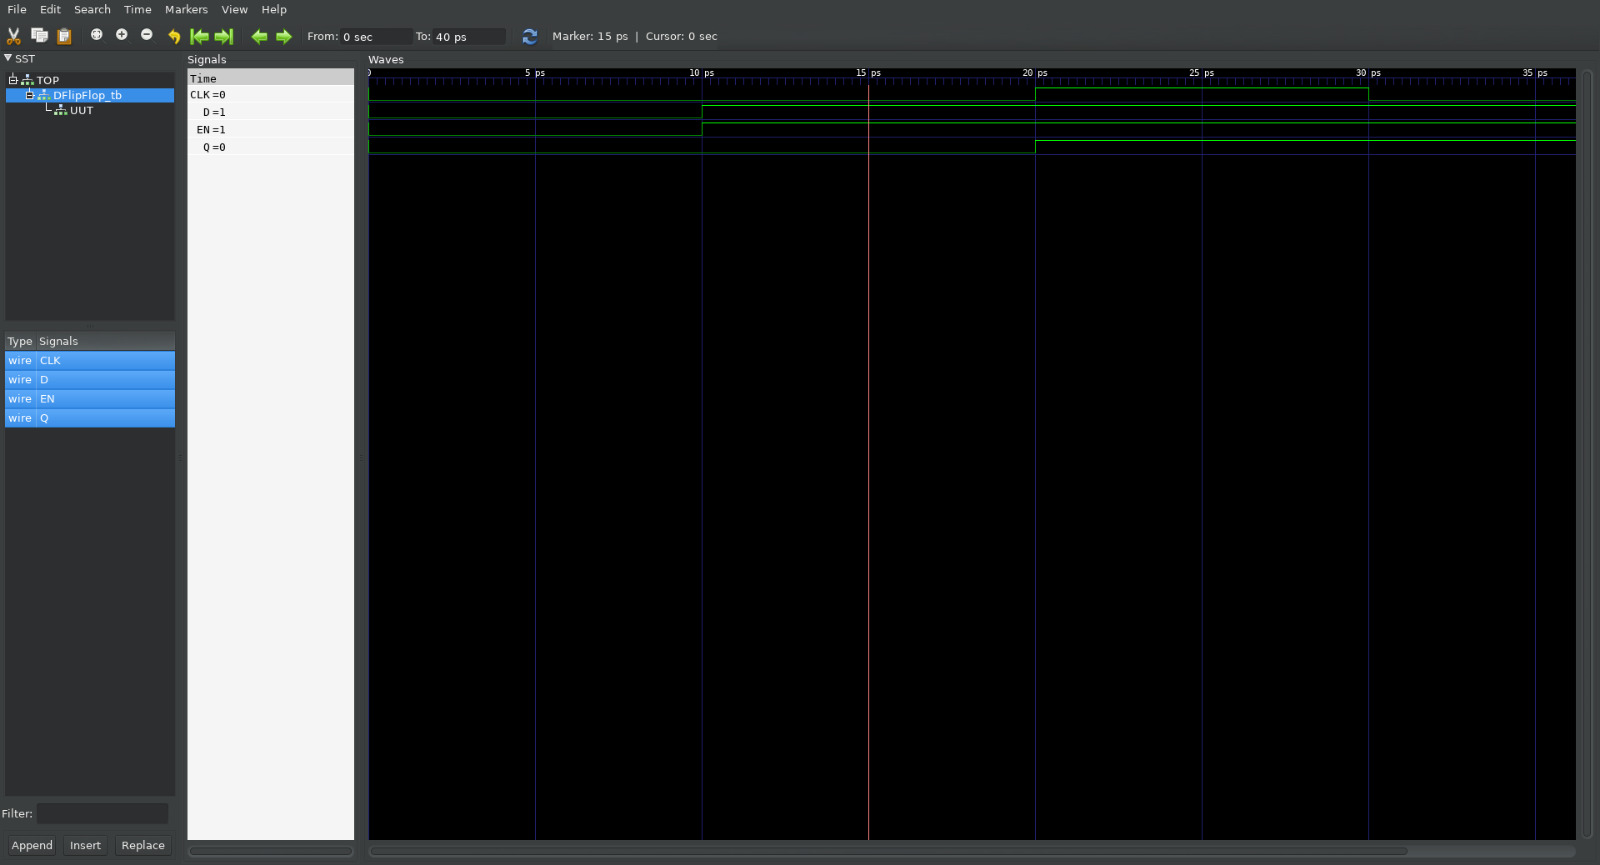
\includegraphics[width=0.95\textwidth]{figures/WhatsApp Image 2023-12-15 at 12.02.26 AM.jpeg}
      \end{center}
      \caption{}
    \end{figure}

    \newpage

  \item A sequential circuit has one flip-flop Q, two inputs x and y, and one
    output S . It consists of a full-adder circuit connected to a D flip-flop,
    as shown in Figure. Write a HDL code for the circuit. 

    \begin{lstlisting}[language=Verilog]
module FullAdderWithFlipFlop (
  input logic x,        // Input x
  input logic y,        // Input y
  input logic clk,      // Clock input
  output logic S        // Output S
);

  logic sum, carry, dff_input;

  always @(posedge clk)
    begin
      // Full Adder logic
      sum = x + y + dff_input;
      carry = (x & y) | ((x ^ y) & dff_input);

      // D Flip-Flop
      dff_input <= carry; // D input is the carry-out from the full-adder
    end

  // Output
  assign S = sum;

endmodule


module FullAdderWithFlipFlop_tb;

  // Inputs
  reg x;
  reg y;
  reg clk;

  // Outputs
  wire S;

  // Instantiate the module under test
  FullAdderWithFlipFlop dut (
    .x(x),
    .y(y),
    .clk(clk),
    .S(S)
  );

  // Clock generation
  always #5 clk = ~clk;

  // Stimulus
  initial begin
    x = 0;
    y = 0;
    clk = 0;

    #10 x = 1;
    #10 y = 1;
    #10 x = 0;
    #10 y = 1;
    #10 x = 1;
    #10 y = 0;
    #10 x = 0;
    #10 y = 0;

    #10 $finish;
  end

  // Monitor
  always @(posedge clk) begin
    $display("x = %b, y = %b, S = %b", x, y, S);
  end

endmodule
    \end{lstlisting}

    \begin{figure}[H]
      \begin{center}
        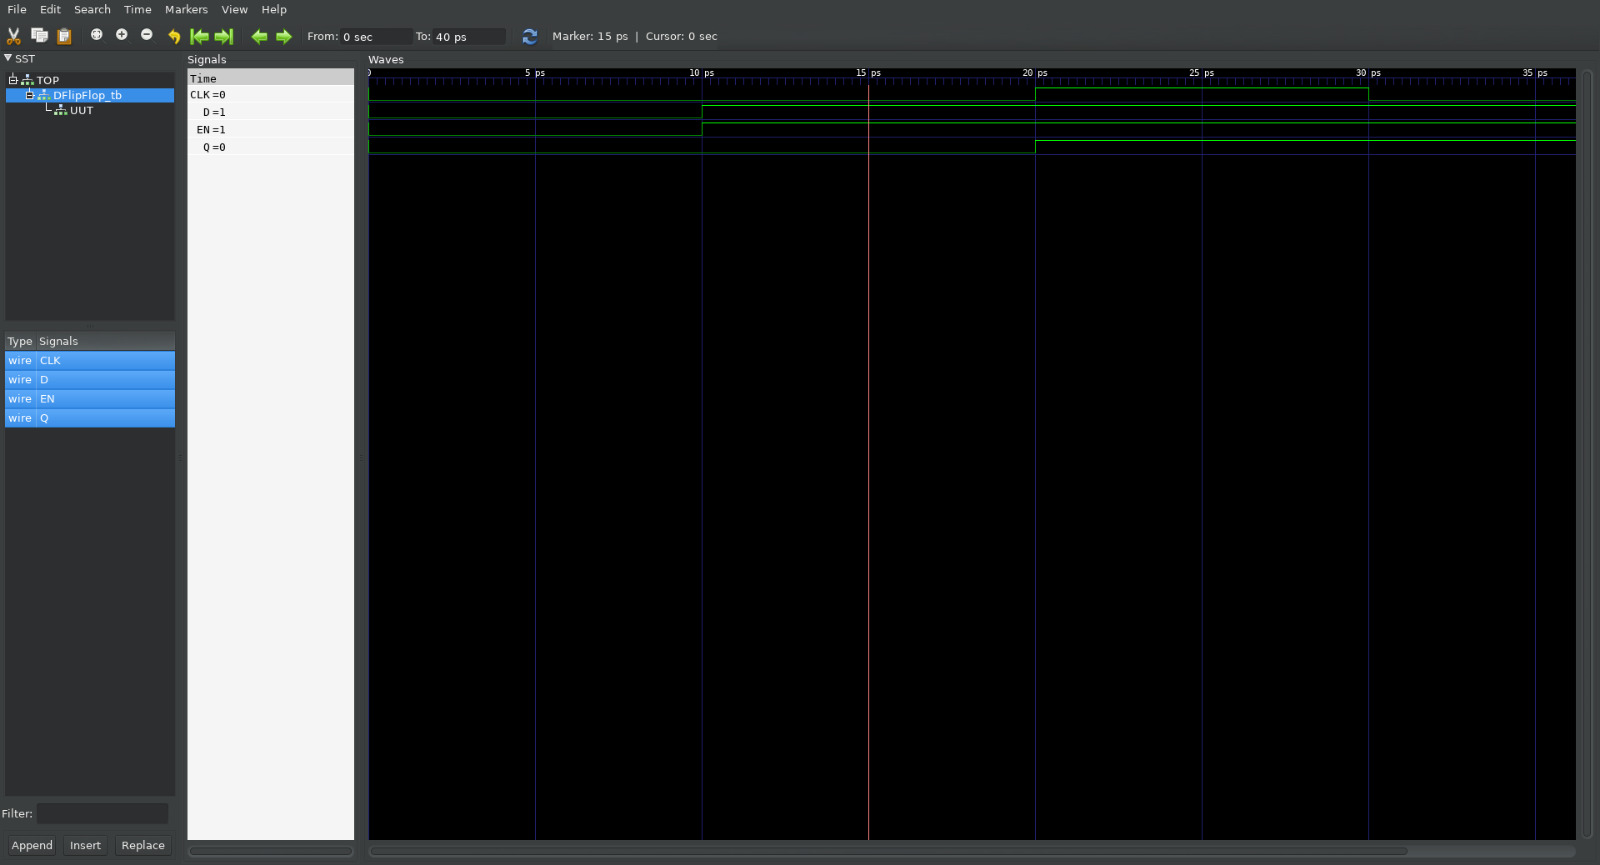
\includegraphics[width=0.95\textwidth]{figures/WhatsApp Image 2023-12-15 at 12.02.26 AM.jpeg}
      \end{center}
      \caption{}
    \end{figure}
    

\end{enumerate}

\end{document}
